%%% Appendix C

\chapter[Appendix C \hspace{0.0025em} Supplementary information for chapter 6]{\textsc{Appendix C} \vspace{8pt} \\ Supplementary information for chapter 6}

\label{appendix:C}

\setcounter{chapter}{0}
\renewcommand{\thechapter}{\Alph{chapter}}
\renewcommand{\theHchapter}{C\thechapter}

\setcounter{section}{0}
\renewcommand{\thesection}{C.\arabic{section}}

\setcounter{figure}{0}
\renewcommand{\thefigure}{C.\arabic{figure}}

\setcounter{table}{0}
\renewcommand{\thetable}{C.\arabic{table}}

\updatemylofappendixC
% \updatemylotappendixC % uncomment this if this appendix has table -> ToC will be updated

\markboth{Appendix C \hspace{0.0025em} Supplementary information for chapter 6}%
{Appendix C \hspace{0.0025em} Supplementary information for chapter 6}

\regularsection
\headerspecialsectionappendix

% ============================================================================================================

\section[micro-PL spectra]{micro-photoluminescence spectra of HVPE-GaN and nanocolumn samples}

This is an additional characterization from \Autoref{subsec:labelsubsec6-2}.

\begin{figure}[H]
    \centering
    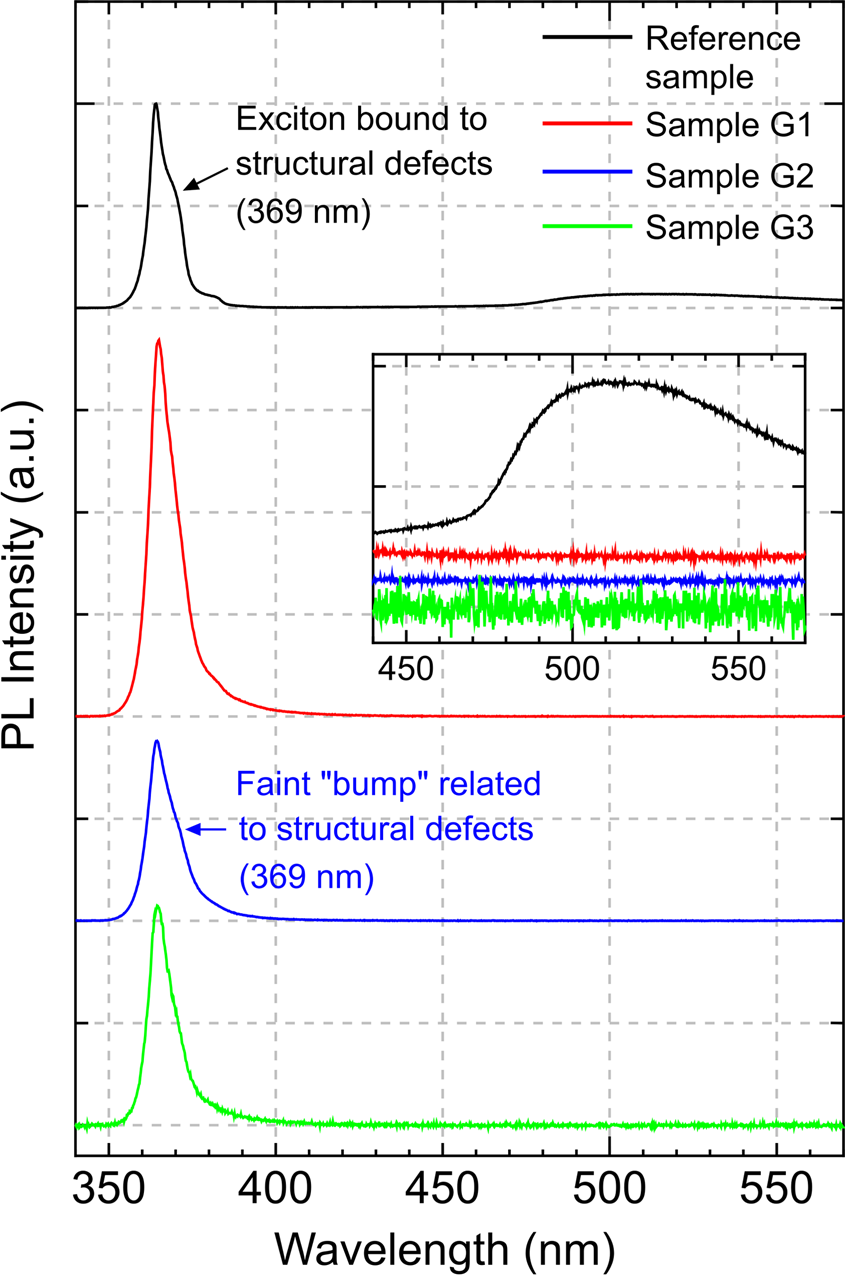
\includegraphics[width=0.6\textwidth]{figures/paper-iv/fig-7.png}
    \caption[RT micro-photoluminescence spectra of reference sample\newline (HVPE-freestanding GaN), samples G1, G2 and G3]{RT micro-photoluminescence spectra of reference sample (HVPE-freestanding GaN), samples G1, G2 and G3. Inset shows the magnified spectra in the wavelength range from 440 to 570 nm, highlighting the presence of broad green and yellow emission band in the reference sample (adapted with permission from ref. \citenum{liudimulyo2020853} \copyright \ Liudi Mulyo \textit{et al}, 2020.}
    \label{fig:figures/paper-iv/fig-7}
\end{figure}

\newpage

\section[micro-Raman spectra]{micro-Raman spectra of pristine graphene and nanocolumn samples after growth}

This is an extra measurement from \autoref{subsec:labelsubsec6-2}

\begin{figure}[H]
    \centering
    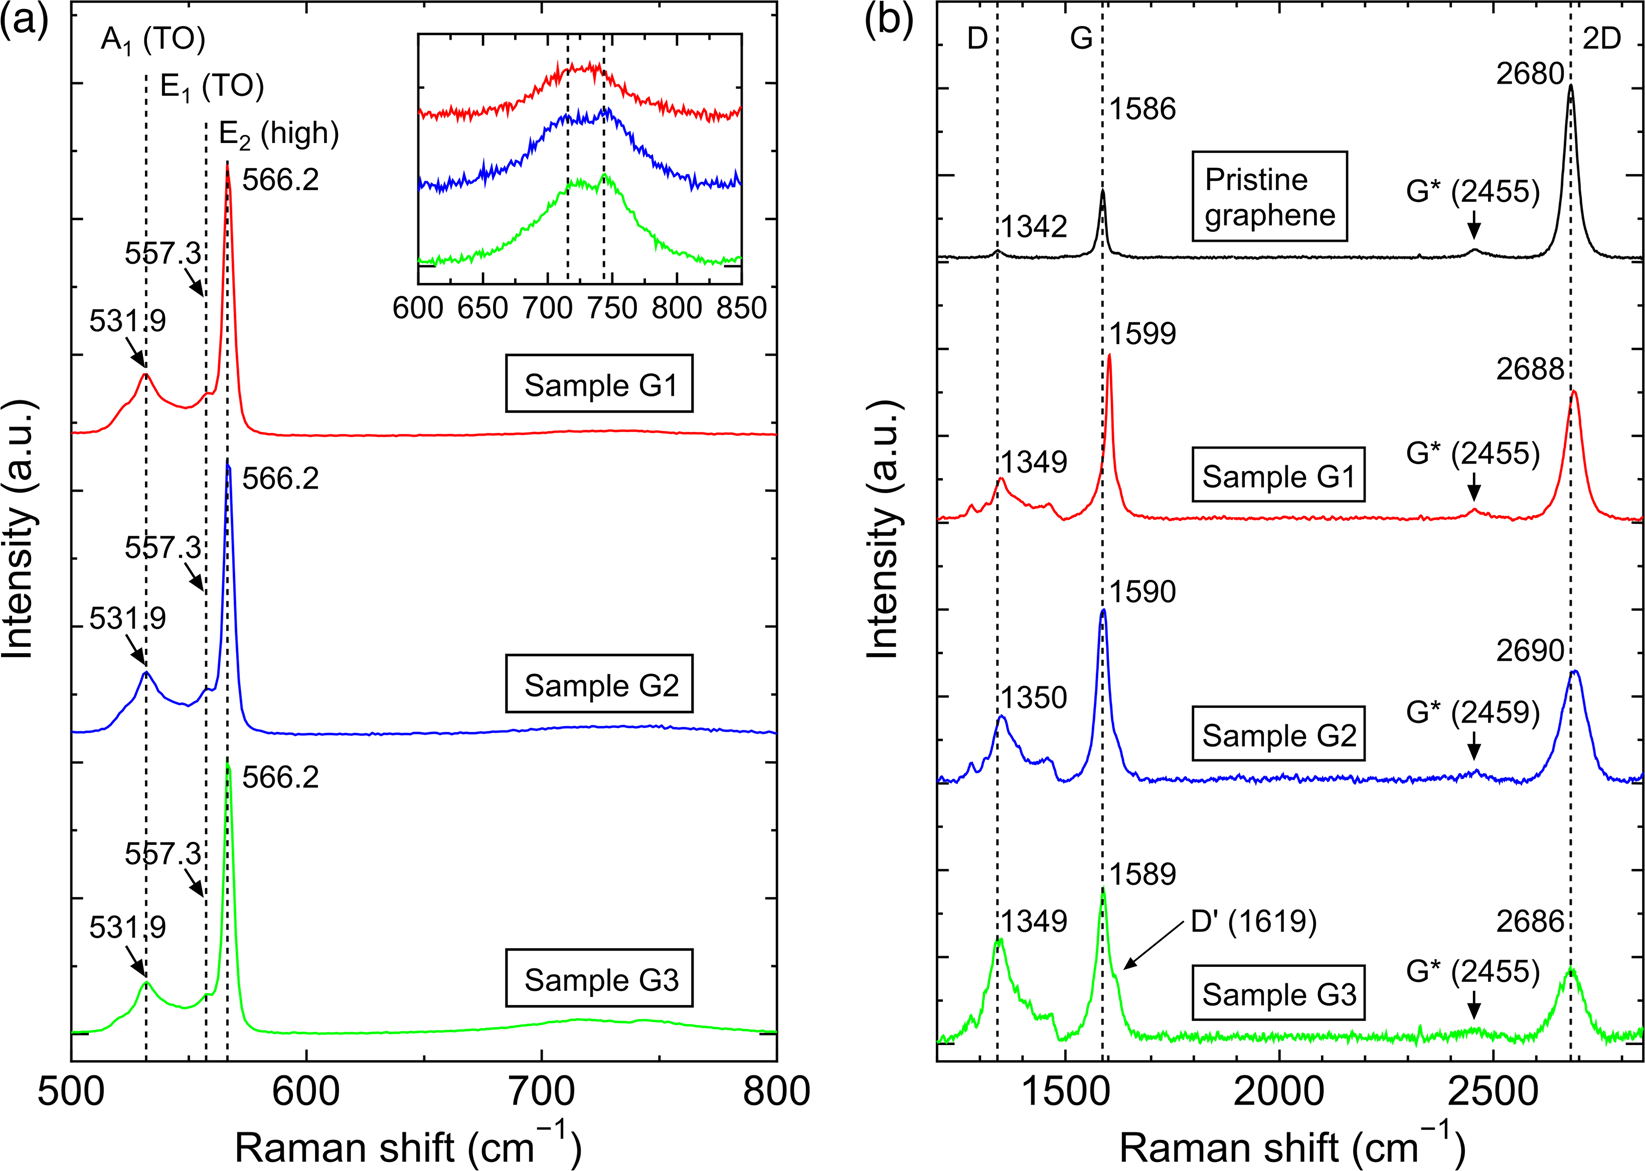
\includegraphics[width=\textwidth]{figures/paper-iv/fig-8.png}
    \caption[Micro-Raman spectroscopy of the nanocolumn samples,\newline including the graphene for each respective sample]{Micro-Raman spectroscopy of the nanocolumn samples, including the graphene for each respective sample. Raman spectra of (\textbf{a}) samples G1, G2 and G3 between 500 and 800 cm\textsuperscript{-1}, with the peak frequencies of the A\textsubscript{1} (TO), E\textsubscript{1} (TO) and E\textsubscript{2} (high) modes indicated by vertical dashed lines (inset: magnification from 600 to 850 cm\textsuperscript{-1}, with the identified peak frequencies at 715 and 743 cm\textsuperscript{-1} of the possible SO and LPP modes, respectively \cite{2016robins,2009jeganathan}, indicated by vertical dashed lines), and (\textbf{b}) pristine graphene, samples G1, G2 and G3 between 1100 and 3200 cm\textsuperscript{-1}. The dashed lines indicate D, G and 2D peak positions of pristine graphene (adapted with permission from ref. \citenum{liudimulyo2020853} \copyright \ Liudi Mulyo \textit{et al}, 2020.}
    \label{fig:figures/paper-iv/fig-8}
\end{figure}

%=======================================================================
%%% References 

\clearpage
\phantomsection
\specialsection
\headerspecialsection

{\hypersetup{urlcolor=ntnu,linkcolor=sophia} % set clickable URL title color to black, not blue like in the main document

\bibliographystyle{unsrtnat-mod} % NATBIB ref style
\bibliography{references}
}

%=======================================================================